\documentclass[iutinfo,a4paper,nocorrections,10pt]{ustl-tdtp}
%\usepackage[utf8]{inputenc}  
%\usepackage[T1]{fontenc}
\usepackage{listings}  
\usepackage{version}

\etablissement{\ustl}
\formation{DUT info 2ème année}
\matiere{Structures de données}
\titre{TD 1 : Étude de quelques tris}
\date{\annee{2018}--\annee{2019}}
%\enseignant{}

\includeversion{solution}
%\excludeversion{solution}

% Include solutions but not questions:
%\excludeversion{question}\includeversion{solution}

\newcommand{\case}{}%\rule[-.40cm]{0pt}{1cm}}
\newcommand{\ident}[3]{(\texttt{#1},~\texttt{#2},~\texttt{#3})}
\newcommand{\rien}{}

\parindent 0cm
\begin{document}
\maketitle
\thispagestyle{empty}

Dans ce TD, vous étudierez et écrirez plusieurs algorithmes de tri classiques. Vous utiliserez la syntaxe du langage Java.


\section{Tri à bulles}

\paragraph{} Le tri à bulles consiste à successivement comparer les cases adjacentes d'un tableaux de valeurs et à les échanger de manière à faire "remonter" les valeurs les plus grandes vers le bout du tableau.
\newline

\textbf{Question 1:} Écrivez la méthode \texttt{static void swap(int [] tab, int idx, int idx2)} qui permet d'échanger deux valeurs d'un tableau d'entiers. Utilisez ensuite cette dernière pour écrire la méthode \texttt{bubbleSort} qui permet de réaliser le tri à bulles. Dans cette première version, vous utiliserez deux boucles for.
\newline
\begin{correction}
{\color{red}
\begin{lstlisting}[language=java]
  static void swap(int [] tab, int idx, int idx2){
	int tmp  = tab[idx];
	tab[idx] = tab[idx2];
	tab[idx2] = tmp;	
    }


\end{lstlisting}

\begin{lstlisting}[language=java]
  static void bubbleSort(int [] tab){	
	for(int i=tab.length-1; i>0; i--){
	  for(int j=0; j<i; j++){
	    if(tab[j]>tab[j+1]){
	     swap(tab,j,j+1);
	    }
	  }
	}
  }
\end{lstlisting}
}
\end{correction}


\textbf{Question 2 :} Appliquez le tri à bulle au tableau de la figure~\ref{tableau}. Que remarquez-vous?
\newline
\begin{correction}
{\color{red}
On constate qu'il y a peu de valeurs à trier et que l'on continue à comparer des valeurs alors que le tableau est déjà trié.
}
\end{correction}

\textbf{Question 3 :} Pour pallier à cela, modifiez le code de la question 1 afin d'éviter tout parcours supplémentaire inutile.
\begin{correction}
{\color{red}

\begin{lstlisting}[language=java]
    static void bubbleSortOpt(int [] tab){
	int end = tab.length - 1;
	while(end > 0){
            int perm = -1; // or if we need all positive numbers
 	    for(int i=0; i<end; i++){
		if(tab[i]>tab[i+1]){
		    swap(tab,i,i+1);
		    perm = i;
		}
	    }
	    end = perm;
	}
    }
  
\end{lstlisting}
}
\end{correction}


\begin{figure}[!h]
\centering
\label{tableau}
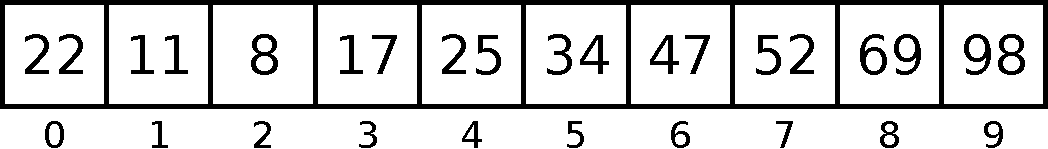
\includegraphics[scale=0.5]{array}
\caption{Tableau d'entiers}
\end{figure}

\textbf{Question 4 :} Combien y a-t-il comparaisons entre les éléments du tableau, effectuées lors de l'exécution de cette fonction dans le pire des cas ? Et combien de permutations?

\begin{correction}
{\color{red}
À chaque itération, il y a n-1 comparaisons et au plus n-1 permutations. Il y a donc exactement $\frac{n \times (n-1)}{2}$ comparaisons et dans le pire cas autant de permutations.
}
\end{correction}

\section{Tri par sélection}

\paragraph{} Le tri par sélection consiste à chaque étape à sélectionner le plus petit élément de la partie du tableau qui n'est pas
encore triée et à l'échanger avec le premier élément de cette partie non triée. Ainsi, au départ la partie non triée du tableau correspond au tableau entier puis elle se rétrécie jusqu'à ne contenir que la dernière case du tableau. \newline


\textbf{Question 5 :} Écrivez les quelques instructions qui permettent de trouver l'indice du plus petit élément d'un tableau \texttt{tab} entre les index \texttt{iBeg} (inclu) et \texttt{iEnd} (exclu). Combien de comparaisons entre les éléments du tableau faut-il faire ?\newline


\begin{correction}
{\color{red}

\begin{lstlisting}[language=java]

	int minIdx = iBeg;

	for(int i = iBeg+1; i<iEnd; i++){
	    if(tab[i] < tab[minIdx]){
		minIdx = i;
	    }
	}


\end{lstlisting}

Il y aura iEnd - iBeg - 1  comparaisons effectuées par la fonction \texttt{minIdx}.
}
\end{correction}


\textbf{Question 6 :} Écrivez une fonction qui fait un tri par sélection sur un tableau d'\texttt{int}, dont le prototype serait le suivant : \texttt{void selectSort(int[] tab)}. Vous pourrez réutiliser la fonction \texttt{swap} définie plus tôt.\newline

\begin{correction}
{\color{red}

\begin{lstlisting}[language=java]
    void selectSort(int [] tab){
	
	int minIdx;
	for(int i=0; i<tab.length; i++){
	    minIdx = i;
	    for(int j=i+1; j<tab.length; j++){
		if(tab[j] < tab[minIdx]){
		    minIdx=j;
		}
	    }
	    if(minIdx!=i){
		swap(tab,i,minIdx);
	    }
	}
    }

\end{lstlisting}
}
\end{correction}

 
\textbf{Question 7 :} Combien y a-t-il comparaisons entre les éléments du tableau, effectuées lors de l'exécution de cette fonction? Et combien de permutations d'éléments du tableau dans le pire des cas?

\begin{correction}

{\color{red}
Le nombre de comparaisons est similaire à celui du tri à bulles. Il y a donc exactement $\frac{n \times (n-1)}{2}$ comparaisons. Dans le pire cas, il y a $n-1$ permutations.

On note que la complexité pire cas du tri par sélection est la même que celle du tri à bulles. Cependant le nombre de permutations est bien moindre.

}

\end{correction}

\section{Tri par insertion}
Le tri par insertion consiste à parcourir le tableau et à chaque étape à insérer l'élément courant à sa place dans le début du tableau déjà trié.\newline


\textbf{Question 8 :} Écrivez les quelques instructions qui permettent d'insérer un élément dans un tableau \texttt{tab} trié. Le tableau est trié entre les bornes \texttt{iBeg} (inclu) et \texttt{iEnd} (exclu), l'élément à insérer est situé à l'index \texttt{iEnd}. Combien de comparaisons faut-il faire? Combien de copies d'éléments?\newline

\begin{correction}
{\color{red}
\begin{lstlisting}[language=java]
	int tmp = tab[iEnd];
	int i = iEnd;
	while(i > iBeg && tab[i-1] >= tmp){
	    tab[i] = tab[i-1];
	    i--;
	}
	tab[i] = tmp;

\end{lstlisting}

Il faut faire iEnd-iBeg comparaisons et autant de copies sont nécessaires dans le pire cas.

}
\end{correction}


\textbf{Question 9 :} Écrivez une fonction qui fait un tri par insertion sur un tableau d'entiers, dont le prototype serait le suivant : \texttt{void insertSort(int[] tab)}\newline
\begin{correction}


{\color{red}

\begin{lstlisting}[language=java]

 void insertSort(int [] tab){
	int tmp,j;
	for(int i = 1; i<tab.length; i++){
	    tmp = tab[i];
	    j = i;
	    while(j > 0 && tab[j-1] >= tmp){
		tab[j] = tab[j-1];
		j--;
	    }
	    tab[j] = tmp;
	}
   }
    
\end{lstlisting}

}
\end{correction}

 
\textbf{Question 10 :} Combien y a-t-il comparaisons entre les éléments du tableau, effectuées lors de l'exécution de cette fonction ? Et combien de copies d'éléments du tableau ?

\begin{correction}

{\color{red}

$\frac{n \times (n-1)}{2}$ comparaisons et copies dans le pire cas.

}
\end{correction}

\section{Fusion de deux tableaux triés}

\textbf{Question 11 :} Écrivez une fonction qui fait la fusion de deux tableaux d'entiers triés, dont le prototype serait le suivant:

\texttt{void fuseTab(int[] tabInA, int[] tabInB, int[] tabOut)}

Le tableau \texttt{tabOut} (préalablement alloué avec une taille suffisante avant l'appel de la fonction \texttt{fuseTab}) doit être trié également et la fonction doit faire un seul "balayage" des tableaux.

\begin{correction}

{\color{red}

\begin{lstlisting}[language=java]
  void fuseTab(int[] tabInA, int[] tabInB, int[] tabOut){

	int aIdx = 0, bIdx = 0, outIdx = 0;
	while(aIdx < tabInA.length && bIdx < tabInB.length){
	    if(tabInA[aIdx] < tabInB[bIdx]){
		tabOut[outIdx++] = tabInA[aIdx++];
	    }else{
		tabOut[outIdx++] = tabInB[bIdx++];
	    }
	}
	while(aIdx < tabInA.length){
	    tabOut[outIdx++] = tabInA[aIdx++]; 
	}
	while(bIdx < tabInB.length){
	    tabOut[outIdx++] = tabInA[bIdx++]; 
	}
    }

\end{lstlisting}

}
\end{correction}
\section{Tri de chaînes de caractères} 


\textbf{Question 12 :} En considérant l'ordre lexicographique, les propositions suivantes sont-elles vraies?

\begin{itemize}
\item[] "glas" < "glasse" \begin{correction}{\color{red}Vrai}\end{correction}
\item[] "voiture" > "moto"   \begin{correction}{\color{red}Vrai}\end{correction}
\item[] "truc" == "curt" \begin{correction}{\color{red}Faux}\end{correction}
\item[] "chapeau" > "char" \begin{correction}{\color{red}Faux}\end{correction}
\end{itemize}
 
\paragraph{} 
 
En Java, la classe \texttt{String} implémente une méthode \texttt{public int compareTo(String anotherString)} de l'interface \texttt{Comparable} qui permet dans le cas des chaînes de comparer deux chaînes de caractères suivant l'ordre lexicographique. La méthode renvoie un entier négatif si l'objet en question précède l'argument dans l'ordre lexicographique, un entier positif si l'objet succède à l'argument et 0 si les deux chaînes sont égales.\newline
 
\textbf{Question 13 :}
L'expression booléenne \texttt{"Abc".compareTo("abc") > 0} est-elle
vraie? 
\begin{correction} {\color{red}Non car la méthode compareTo se base
    sur la valeur des caractères dans la table unicocde où la valeur
    d'une lettre majuscule est inférieure à celle de la même lettre en
    minuscule. Donc la valeur de retour est un entier négatif.
    Remarque : la table unicode est une extension de la table
    ascii.}
\end{correction}

\textbf{Question 14 :} Modifiez l'algorithme de tri de façon à trier un tableau de chaînes de caractères, la méthode aura donc le prototype suivant : \texttt{void insertSort(String [] tab)}.

\begin{correction}


{\color{red}

\begin{lstlisting}[language=java]

 void insertSort(String [] tab){
	String tmp;	
	int j;
	for(int i = 1; i<tab.length; i++){
	    tmp = tab[i];
	    j = i;
	    while(j > 0 && tab[j-1].compareTo(tmp)>=0){
		tab[j] = tab[j-1];
		j--;
	    }
	    tab[j] = tmp;
	}
   }
    
\end{lstlisting}

}
\end{correction}


\end{document}

